\documentclass[14pt]{article}
\usepackage{graphicx}
\usepackage[left=3cm, right=1.5cm, top=1.5cm, bottom=2cm]{geometry}
\usepackage[russian]{babel}
\usepackage[T2A]{fontenc}
\usepackage[utf8]{inputenc}
\usepackage[unicode]{hyperref}
\usepackage{a4wide}
\usepackage{pdfpages}

\begin{document}

\includepdf[pages=-]{title_Ali.pdf}
\clearpage
\tableofcontents
\clearpage
\section{Команда}
\section{Ресурсы}
	\subsection{Сетевой график}
	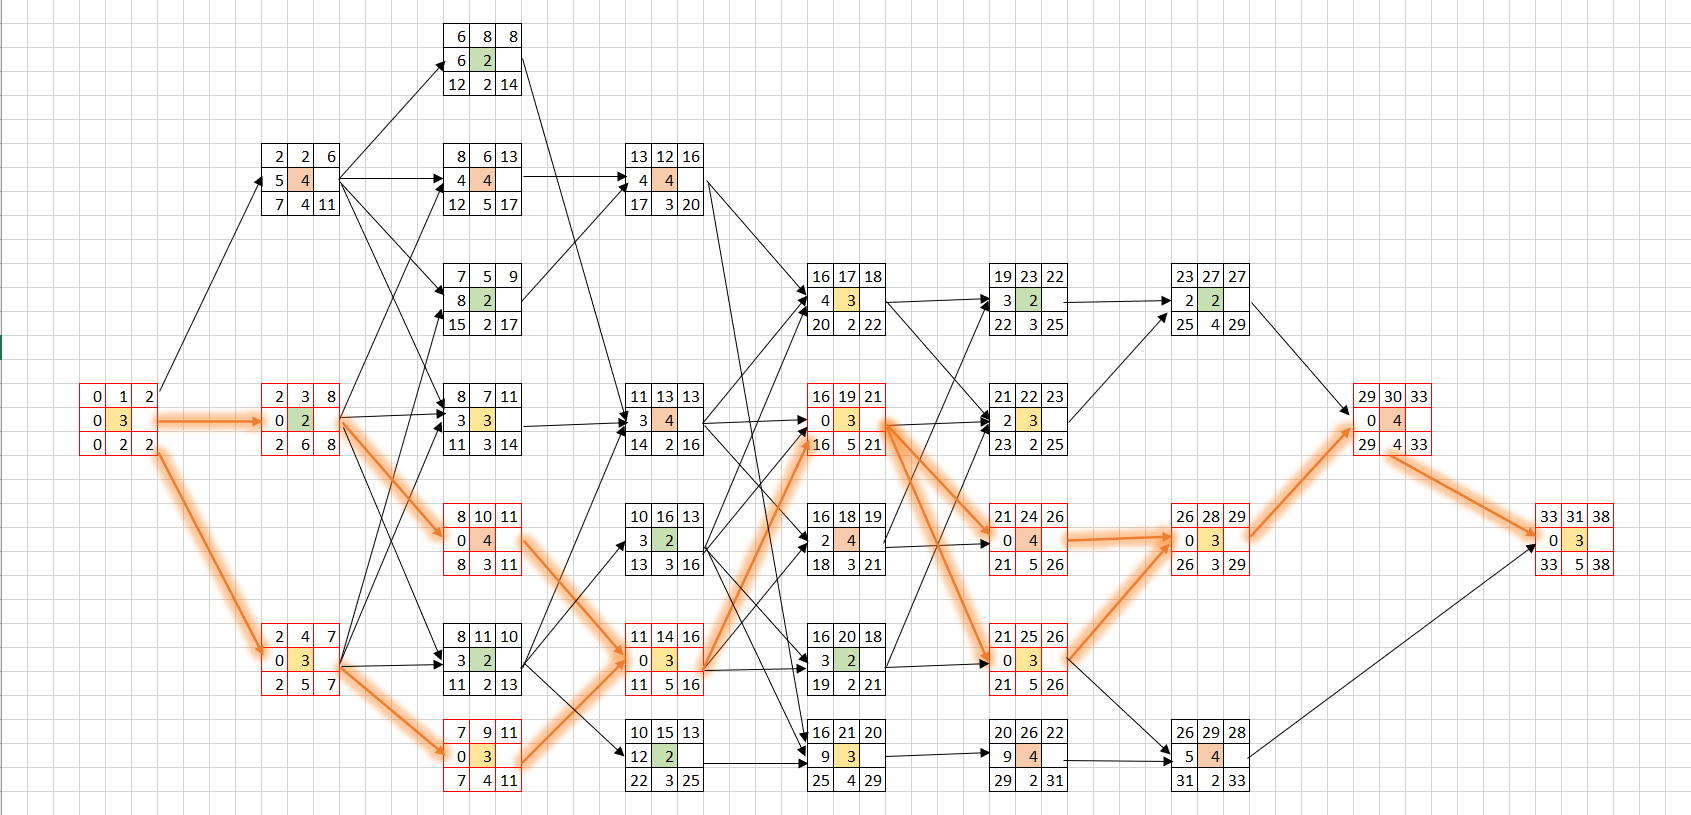
\includegraphics[width=\textwidth]{../img/init_network_graph.png}\\
	В проекте 4 попарно различных кретических пути.
	\subsection{Назначение ресурсов}
	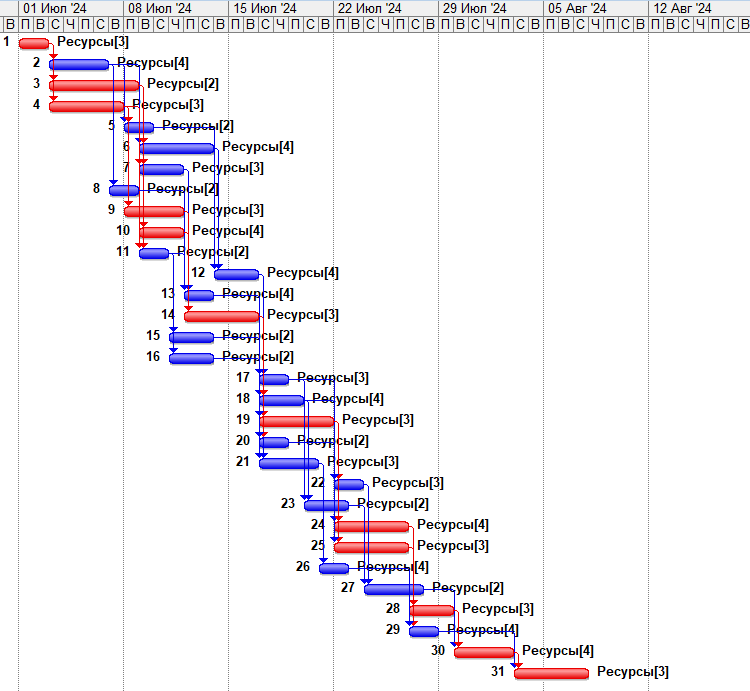
\includegraphics[width=\textwidth]{../img/init_resource_manage.png}
\section{Задача}
	Попробовать уменьшить количество используемых ресурсов до 5 в день,
		меняя при этом количество ресурсов не более чем на 2 единицы.
	Дата окончания проекта может меняться.
\section{Решение}
	Основную проблему здесь являются <<Четвёрки>> из-за невозможности их делать паралельно другой задаче (См первый отчёт).
	Поэтому одной из лучших тактик является превратить все мешающие Четвёрки в <<Тройки>> или <<Двойки>> по мере необходимости.
		\subsection{Первый вариант}
		Свобода в дате окончания проекта позволила обойтись минимальными изменениями.
		Обращаю внимание на то, что проект заканчивается \texttt{28.08}!\\
		{\LARGE Что поменяли:}\\
		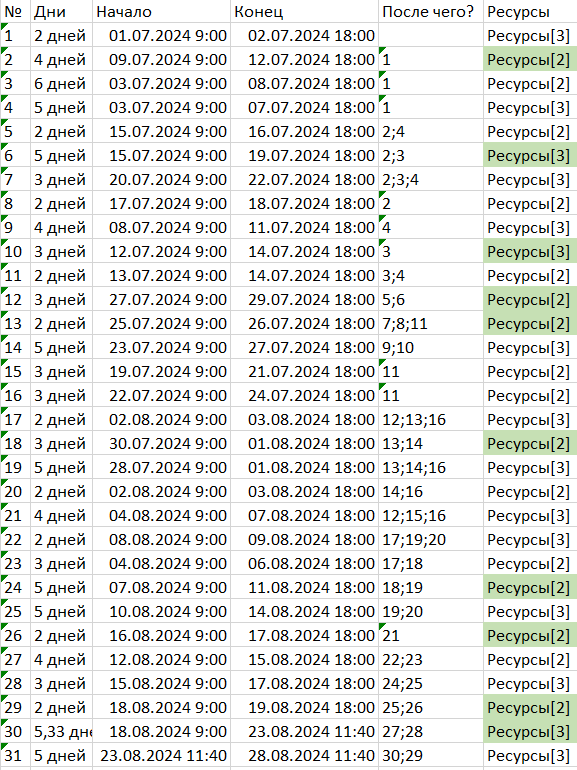
\includegraphics[height=0.6\textheight]{../img/2b1_days_change.png}\\ 
		{\LARGE Как это выглядит:}\\
		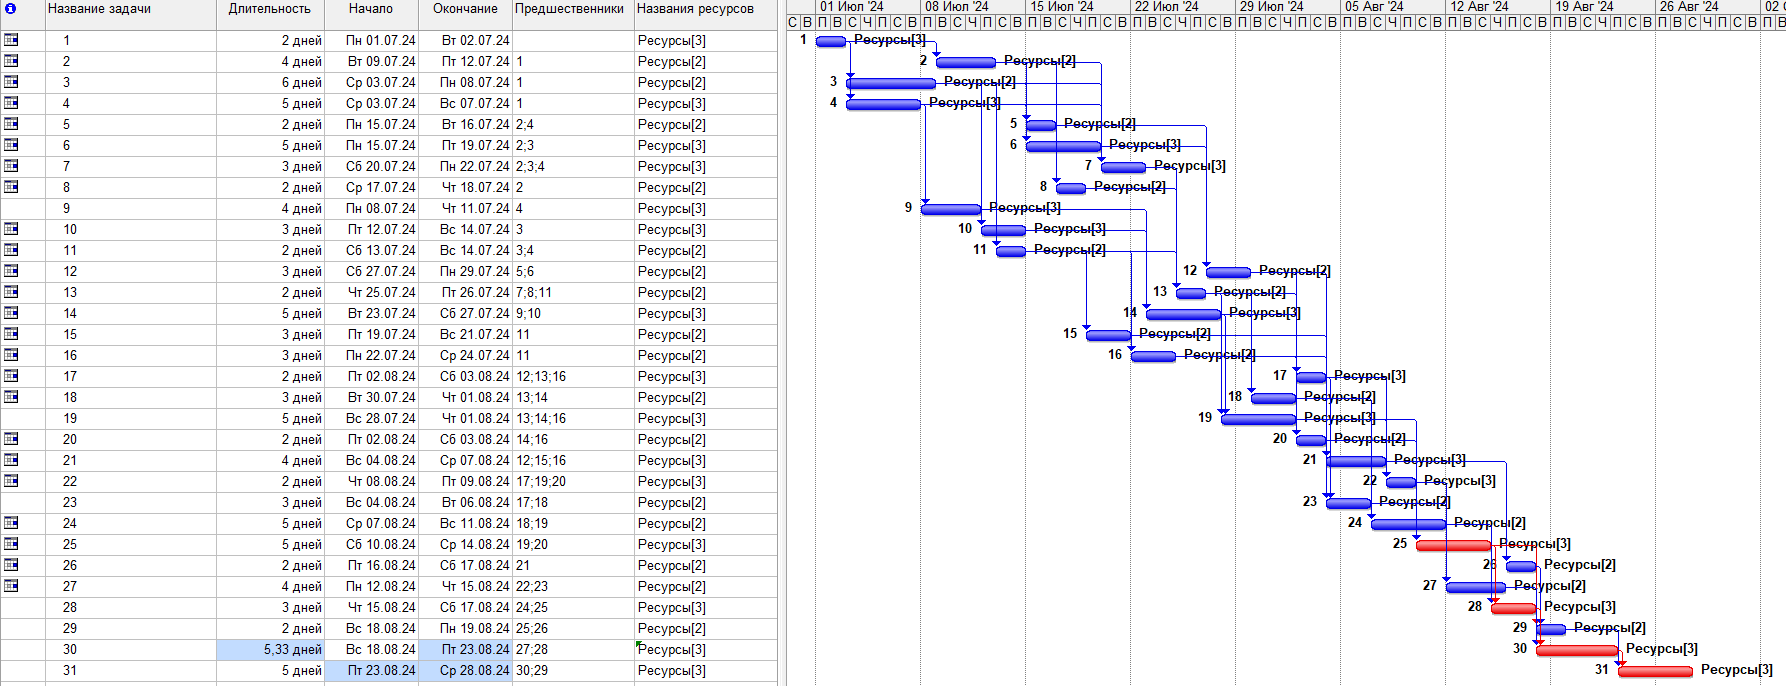
\includegraphics[width=\textwidth]{../img/ot2b1_1.png}\\
		Такая стратегия позволяет выолнить не более двух задач за раз.
		Конкретно в этом случаев каждый день выполняются ровно две задачи.
		Исключением является <<особые>> задачи (см отчёт первого задания)
		{\LARGE Cколько оно тратит:}\\
		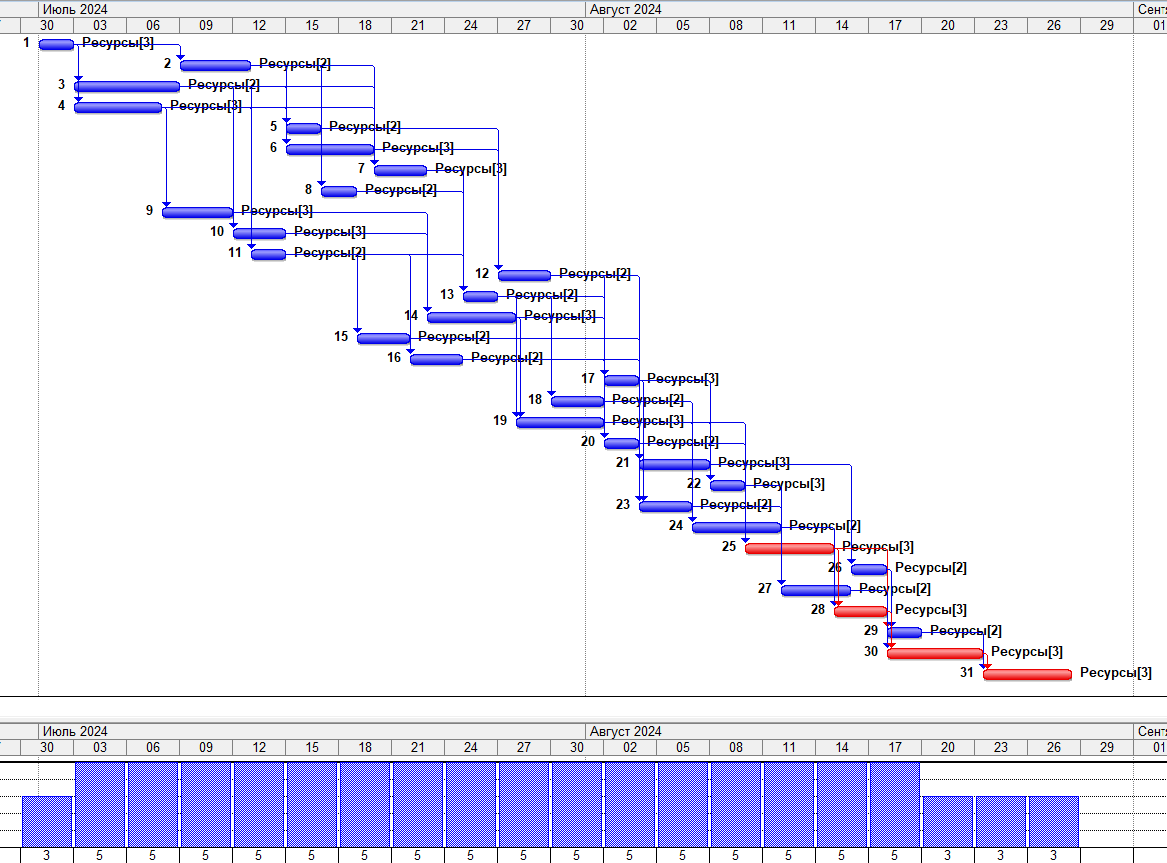
\includegraphics[width=\textwidth]{../img/2b1_answer.png}\\ 
	\subsection{Второй вариант}
		Теперь попробуем уменьшить дату окончания проекта.
		Для этого придётся внести больше изменений в задачи.
		Опишем новую тактику.
		Если раньше мы создавали 2 линии (из троек и двоек),
			то теперь мы создаём 3 линии (из двух двоек и одной единицы)
		Это позволит выполняться сразу 3-м задачам одновременно
		Новая дата окончания: \texttt{13.08}.\\
		{\LARGE Что поменяли:}\\
		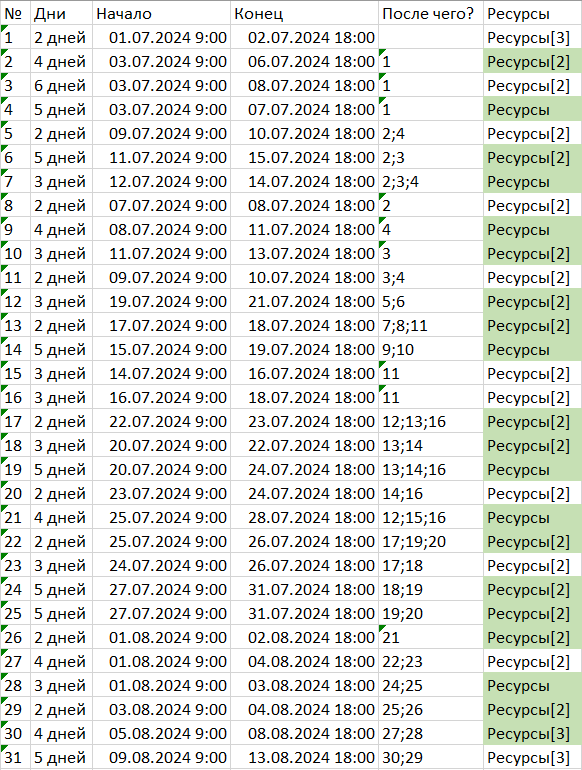
\includegraphics[height=0.6\textheight]{../img/2b2_days_change.png}\\ 
		{\LARGE Как это выглядит:}\\
		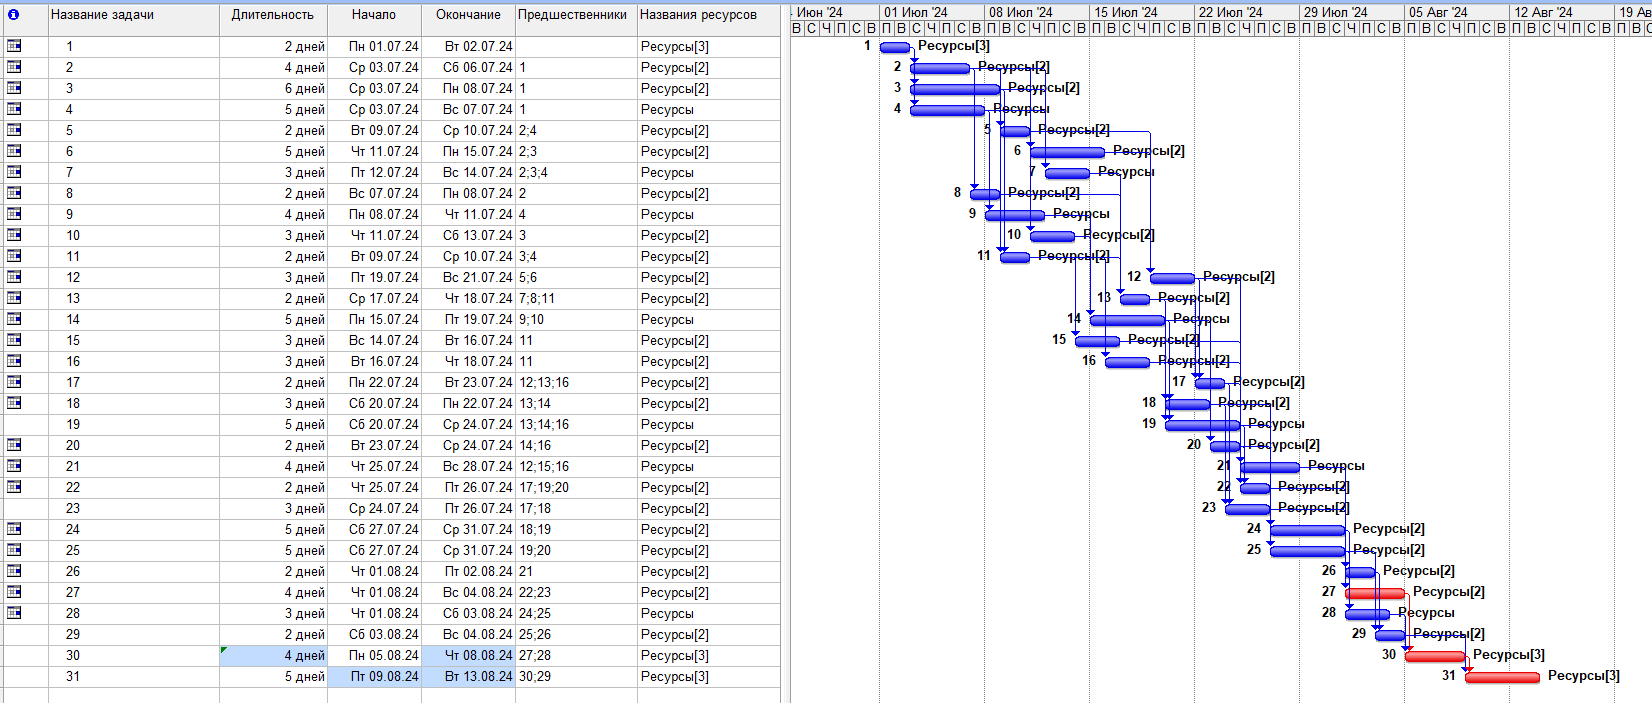
\includegraphics[width=\textwidth]{../img/ot2b2_1.png}\\
		{\LARGE Cколько оно тратит:}\\
		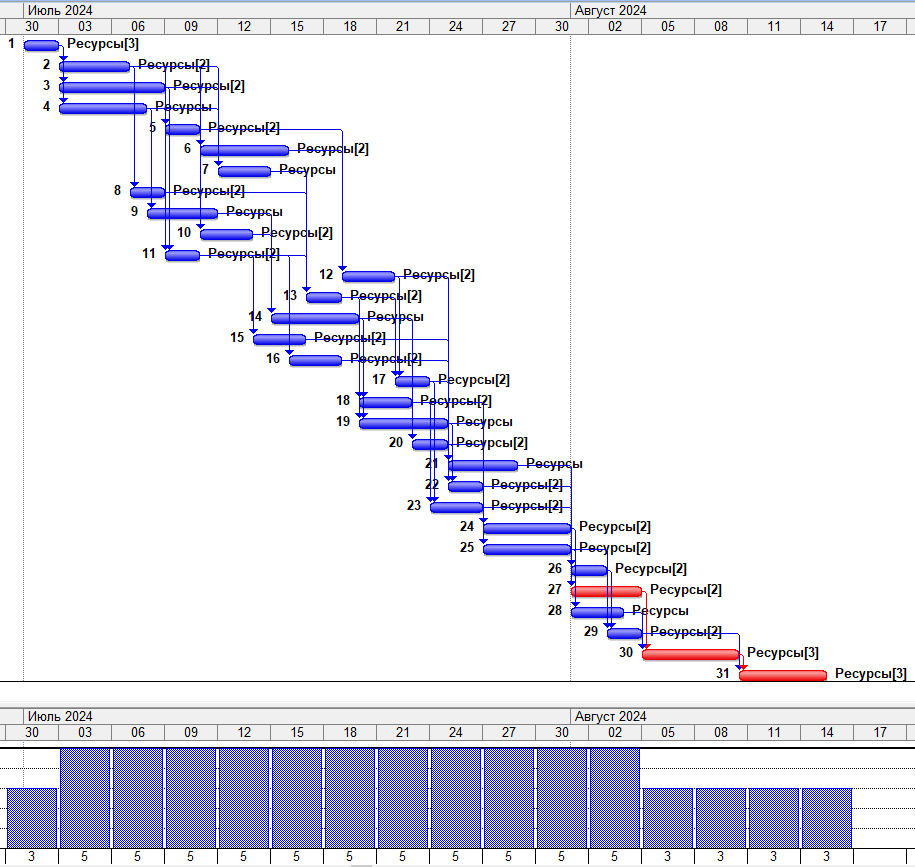
\includegraphics[width=\textwidth]{../img/2b2_answer.png}\\ 
	\subsection{Третий вариант}
		Попробуем получить ещё более лучшую дату окончания.
		Сделаем это по аналоги с прошлым пунктом.
		Мы уменьшим ресурсы некогорых двоек на одну единицу.
		Таким образом, мы сможем умещать 4 задачи в день.
		Единственная проблема в том, что случаи когда 4 задачи решаются в один день невероятно редки,
			поэтому выигрыш по времени незначителен.
		В этом варианте была достигнута дата \texttt{12.08}.
		{\LARGE Что поменяли:}\\
		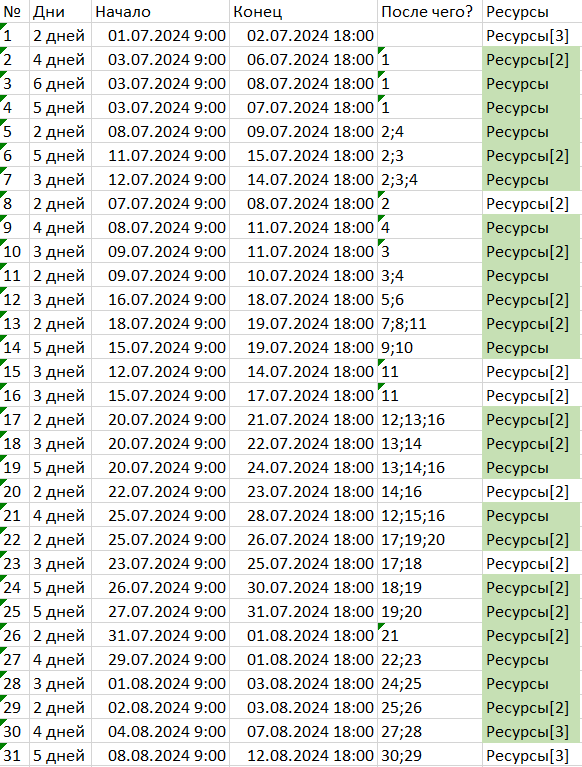
\includegraphics[height=0.6\textheight]{../img/2b3_days_change.png}\\ 
		{\LARGE Как это выглядит и сколько оно тратит:}\\
		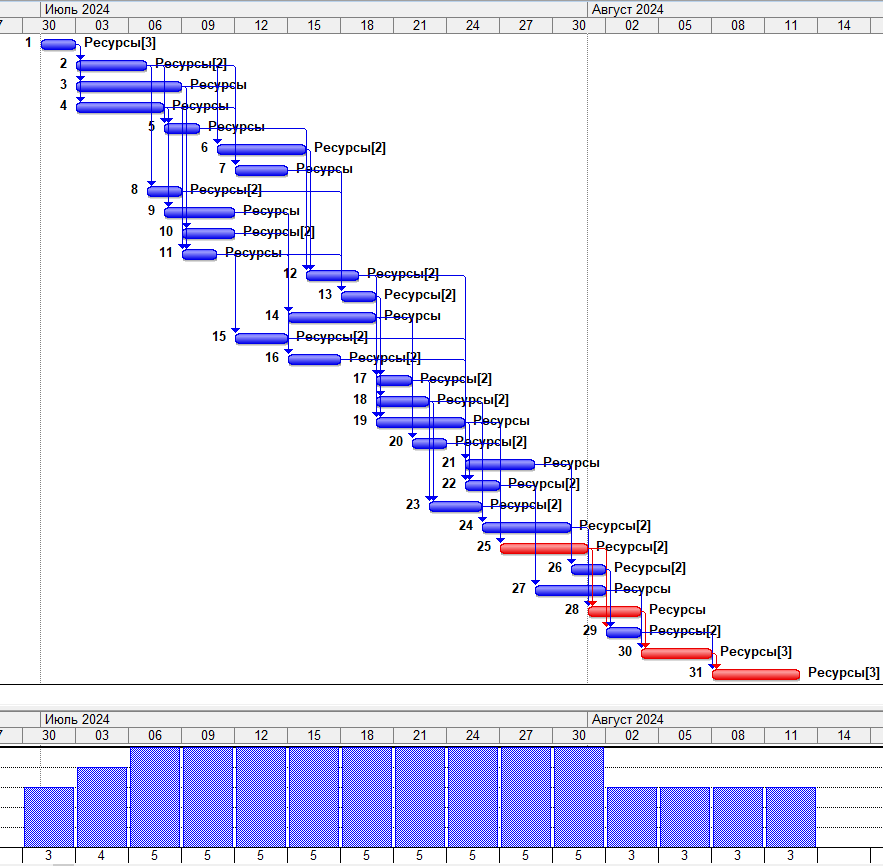
\includegraphics[width=\textwidth]{../img/2b3_answer.png}\\ 
\end{document}
